\documentclass[14pt,xcolor=pdftex,dvipsnames,table]{beamer}\usepackage[]{graphicx}\usepackage[]{color}
%% maxwidth is the original width if it is less than linewidth
%% otherwise use linewidth (to make sure the graphics do not exceed the margin)
\makeatletter
\def\maxwidth{ %
  \ifdim\Gin@nat@width>\linewidth
    \linewidth
  \else
    \Gin@nat@width
  \fi
}
\makeatother

\definecolor{fgcolor}{rgb}{0.345, 0.345, 0.345}
\newcommand{\hlnum}[1]{\textcolor[rgb]{0.686,0.059,0.569}{#1}}%
\newcommand{\hlstr}[1]{\textcolor[rgb]{0.192,0.494,0.8}{#1}}%
\newcommand{\hlcom}[1]{\textcolor[rgb]{0.678,0.584,0.686}{\textit{#1}}}%
\newcommand{\hlopt}[1]{\textcolor[rgb]{0,0,0}{#1}}%
\newcommand{\hlstd}[1]{\textcolor[rgb]{0.345,0.345,0.345}{#1}}%
\newcommand{\hlkwa}[1]{\textcolor[rgb]{0.161,0.373,0.58}{\textbf{#1}}}%
\newcommand{\hlkwb}[1]{\textcolor[rgb]{0.69,0.353,0.396}{#1}}%
\newcommand{\hlkwc}[1]{\textcolor[rgb]{0.333,0.667,0.333}{#1}}%
\newcommand{\hlkwd}[1]{\textcolor[rgb]{0.737,0.353,0.396}{\textbf{#1}}}%

\usepackage{framed}
\makeatletter
\newenvironment{kframe}{%
 \def\at@end@of@kframe{}%
 \ifinner\ifhmode%
  \def\at@end@of@kframe{\end{minipage}}%
  \begin{minipage}{\columnwidth}%
 \fi\fi%
 \def\FrameCommand##1{\hskip\@totalleftmargin \hskip-\fboxsep
 \colorbox{shadecolor}{##1}\hskip-\fboxsep
     % There is no \\@totalrightmargin, so:
     \hskip-\linewidth \hskip-\@totalleftmargin \hskip\columnwidth}%
 \MakeFramed {\advance\hsize-\width
   \@totalleftmargin\z@ \linewidth\hsize
   \@setminipage}}%
 {\par\unskip\endMakeFramed%
 \at@end@of@kframe}
\makeatother

\definecolor{shadecolor}{rgb}{.97, .97, .97}
\definecolor{messagecolor}{rgb}{0, 0, 0}
\definecolor{warningcolor}{rgb}{1, 0, 1}
\definecolor{errorcolor}{rgb}{1, 0, 0}
\newenvironment{knitrout}{}{} % an empty environment to be redefined in TeX

\usepackage{alltt}

% Specify theme
\usetheme{Madrid}
% See deic.uab.es/~iblanes/beamer_gallery/index_by_theme.html for other themes
\usepackage{caption}
\usepackage{tikz}
\usepackage{multirow}
% Specify base color
\usecolortheme[named=OliveGreen]{structure}
% See http://goo.gl/p0Phn for other colors

% Specify other colors and options as required
\setbeamercolor{alerted text}{fg=Maroon}
\setbeamertemplate{items}[square]

% Title and author information
\title{Elasticity}
\author{Rob Hayward}
\IfFileExists{upquote.sty}{\usepackage{upquote}}{}
\begin{document}

\begin{frame}
\titlepage
\end{frame}


\section{Classsic analysis of consumer behaviour}
\begin{frame}{Introduction}
Economic man will make rational choice.  
\begin{itemize}[<+-| alert@+>]
\item Diminishing marginal utility
\item Demand for one product
\item Demand for two or more produdcts
\item Effect of price or income changes
\item Infference analysis
\end{itemize}
\end{frame}

\begin{frame}{Indifference}
\begin{columns}[T]
\begin{column}{0.48\textwidth}
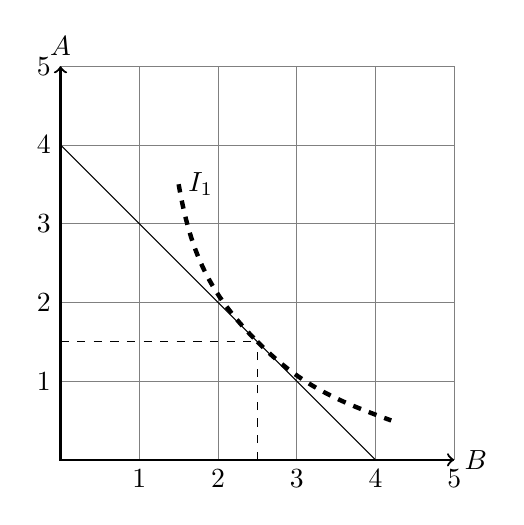
\begin{tikzpicture}
\draw [help lines] (0, 0) grid (5, 5);
\draw [<->, thick] (0, 5) node (yaxis) [above] {$A$} 
  |- (5, 0) node (xaxis) [right] {$B$};;
\draw (4, 0) -- (0, 4);
\draw [dashed, ultra thick] (1.5, 3.5) to [out = -80, in = 135] (2.5, 1.5);
\draw [dashed, ultra thick] (2.5, 1.5) to [out = -45, in = 160] (4.2, 0.5);
\node [below] at (1, 0)  {1};
\node [below] at (2, 0) {2};
\node [below] at (3, 0) {3};
\node [below] at (4, 0) {4};
\node [below] at (5, 0) {5};
\node [left] at (0, 1) {1};
\node [left] at (0, 2) {2};
\node [left] at (0, 3) {3};
\node [left] at (0, 4) {4};
\node [left] at (0, 5) {5};
\node [right] at (1.5, 3.5) {$I_1$};
\pause
\draw [dashed, thin] (2.5, 0) to (2.5, 1.5);
\draw [dashed, thin] (0, 1.5) to (2.5, 1.5);
\end{tikzpicture}
\end{column}
\begin{column}{0.48\linewidth}
There are two products 
\begin{itemize}
\item Price of (A) = 3
\item Price of (B) = 3
\item Budget = 12
\item Can buy $\frac{12}{3} = 4A$
\item Can buy $\frac{12}{3} = 4B$
\end{itemize}
\begin{equation*}
I_1 = \frac{MU_A}{MU_B}
\end{equation*}
\end{column}
\end{columns}
\end{frame}


\begin{frame}{Price increase}
\begin{columns}[T]
\begin{column}{0.48\textwidth}
\begin{tikzpicture}
\draw [help lines] (0, 0) grid (5, 5);
\draw [<->, thick] (0, 5) node (yaxis) [above] {$A$} 
  |- (5, 0) node (xaxis) [right] {$B$};;
\draw [dashed, ultra thick] (1.5, 3.5) to [out = -80, in = 135] (2.5, 1.5);
\draw [dashed, ultra thick] (2.5, 1.5) to [out = -45, in = 160] (4.2, 0.5);
\draw (4, 0) -- (0, 4)[]
\node [below] at (1, 0)  {1};
\node [below] at (2, 0) {2};
\node [below] at (3, 0) {3};
\node [below] at (4, 0) {4};
\node [below] at (5, 0) {5};
\node [left] at (0, 1) {1};
\node [left] at (0, 2) {2};
\node [left] at (0, 3) {3};
\node [left] at (0, 4) {4};
\node [left] at (0, 5) {5};
\node [right] at (1.5, 3.5) {$I_1$};
\pause
\draw (3, 0) -- (0, 4);
\draw [dashed, ultra thick] (1.5, 3.5) to [out = -80, in = 135] (2.0, 1.5);
\draw [dashed, ultra thick] (2.0 1.5) to [out = -45, in = 160] (4.2, 0.5);
\end{tikzpicture}
\end{column}
\begin{column}{0.48\linewidth}
There are two products 
\begin{itemize}
\item Price of (A) = 3
\item Price of (B) = 4
\item Budget = 12
\item Can buy $\frac{12}{3} = 4A$
\item Can buy $\frac{12}{4} = 3B$
\end{itemize}
\begin{equation*}
I_1 = \frac{MU_A}{MU_B}
\end{equation*}
\end{column}
\end{columns}
\end{frame}

\end{document}

